\documentclass[a4paper, 12pt]{article}

\usepackage[T2A]{fontenc}
\usepackage[utf8]{inputenc}
\usepackage[english,russian]{babel}
\usepackage[left=15mm, top=20mm, right=15mm, bottom=20mm, nohead, nofoot]{geometry}

\usepackage{hyperref}
\usepackage{graphicx}
\usepackage{wrapfig}
\usepackage{afterpage}
\usepackage{amsmath, amsfonts, amssymb, amsthm, mathtools}
\author{Хомутов Андрей, группа Б06-903}
\title{ВПВ по курсу "Электричество и магнетизм" \\ Конденсатор на высоких частотах}
\date{22 декабря 2020 г.}
%%%%%%%%%%%%%%%%%%%%%%%%%%%%%%%%%%%%%%%%%%%%%%%%%%%%%%%%%%%%%%%%%%%%%%%%%
\usepackage{graphicx, wrapfig, subcaption, setspace, booktabs}
\usepackage[protrusion=true, expansion=true]{microtype}
\usepackage[english]{babel}
\usepackage{sectsty}
\usepackage{url, lipsum}
\newcommand{\HRule}[1]{\rule{\linewidth}{#1}}
\onehalfspacing
\setcounter{tocdepth}{5}
\setcounter{secnumdepth}{5}
%%%%%%%%%%%%%%%%%%%%%%%%%%%%%%%%%%%%%%%%%%%%%%%%%%%%%%%%%%%%%%%%%%%%%%%%%


\begin{document}

\title{ \normalsize \textsc{Лабораторная работа по общей физике}
		\\ [4.0cm]
		\HRule{0.5pt} \\ [0.3cm]
		\LARGE \textbf{{Разрешающая способность}}
		\HRule{0.5pt} \\ [0.1cm]
		\normalsize  \vspace*{18\baselineskip}}

\date{}

\author{%Шамарина Екатерина, Б06-903 \\
		Хомутов Андрей, Б06-903 \\
ФБМФ, 2021\\ }

\maketitle
\thispagestyle{empty}
\newpage
%%%%%%%%%%%%%%%%%%%%%%%%%%%%%%%%%%%%%%%%%%%%%%%%%%%%%%%%%%%%%%%%%%%%%%%%%
%\section*{Цели работы} 

%%%%%%%%%%%%%%%%%%%%%%%%%%%%%%%%%%%%%%%%%%%%%%%%%%%%%%%%%%%%%%%%%%%%%%%%%
 
%\section{Теоретическая часть}
%\subsection{...}

%\subsubsection{...}

\section{Практическая часть}
\subsection{Определение периодов решеток по их пространственному спектру}
Длина волны излучения лазера $\lambda=532$ нм (зеленый). По измеренному расстоянию между максимумами можно определить период решетки $d=\frac{nH}{sin(\varphi)}$. Соответсвущие измерения и расчеты приведены в таблице 1.
\begin{table}[h]
\begin{center}
\caption{Расчет периода решеток}
\begin{tabular}{|c|c|c|c|c|c|c|}
\hline
Решетка & Н, см & $\Delta x$   & $sin(\varphi)$ & n  & d, мкм &  $\delta_{d},$ мкм   \\ \hline
1         & 120   & 194 & 0,080     & 3  & 20,0   & 0,4 \\ \hline
2         & 120   & 214 & 0,088     & 5  & 30,3   & 0,5 \\ \hline
3         & 120   & 215 & 0,088     & 10 & 60,3   & 1,1 \\ \hline
4         & 120   & 109 & 0,045     & 10 & 118    & 3   \\ \hline
5         & 120   & 161 & 0,066     & 20 & 160    & 3   \\ \hline
волос     & 144   & 89  & 0,031     & 5  & 86,2   & 2,7 \\ \hline
\end{tabular}
\end{center}
\end{table} % таблица 1

\subsection{Определение периодов решеток по изображению, увеличенному с помощью микроскопа}
Соберем модель проекционного микроскопа (см. рис. 1), отцентрируем ее и настроим. Далее измерим соответствующие параметры установки и рассчитаем периоды решеток. Значения и расчеты представлены в таблице 2. Период вычисляем как $d = \frac{\Delta x}{kN}, N =
\frac{b_{1} b_{2}}{a_{1} a_{2}}$.
\begin{figure}[h!]
    \begin{center}
    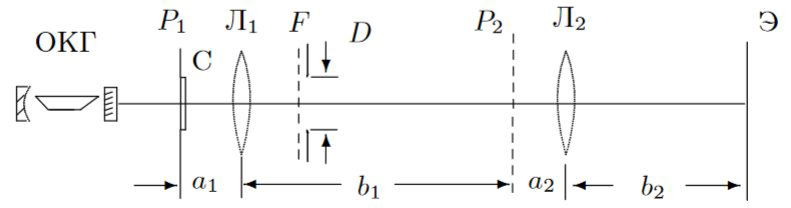
\includegraphics[width=0.8\textwidth]{ust.png}
    \end{center}
    \caption{Схема экспериментальной установки}
\end{figure} %рисунок установки 1

\begin{table}[h]
\begin{center}
\caption{Период решетки через увеличение микроскопа}
\begin{tabular}{|c|c|c|c|c|c|c|c|c|}
\hline
Решетка & a1, мм  & b1, мм   & a2, мм & b2, мм  & $\Delta x$, мм   & k  & d, мкм    & $\delta_{d},$ мкм   \\ \hline
1         & 135 & 1050 & 25 & 370 & 100 & 43 & 20,2  & 0,5 \\ \hline
2         & 135 & 1050 & 25 & 370 & 100 & 29 & 30,0  & 0,7 \\ \hline
3         & 135 & 1050 & 25 & 370 & 110 & 16 & 59,7  & 1,4 \\ \hline
4         & 135 & 1050 & 25 & 370 & 110 & 8  & 119,4 & 2,9 \\ \hline
5         & 135 & 1050 & 25 & 370 & 110 & 6  & 159   & 4   \\ \hline
\end{tabular}
\end{center}
\end{table}
Как видим, результаты обоих методик идентичны (более того, результаты 20, 30, 60, 120, 160 мкм естественны), а значит они обе одинаково хорошо пригодны для определения периодов дифракционных решеток.

\subsection{Определение периодов решеток по оценке разрешающей способности микроскопа}

Минимальное разрешаемое объективом микроскопа расстояние определяется условием
$$\ell_{\min } \approx \frac{\lambda}{\sin A} \approx \frac{\lambda}{D / 2 f},$$
где $D$ - диаметр диафрагмы, $A$ - апертура.


\subsection{Пространственная фильтрация и мультиплицирование}
При фильтрации с помощью щели, мы будем наблюдать различные картины при изменении ориентации щели. Для вертикальной щели -  вертикальные полосы, для горизонтальной - горизонатльные, для наклоненной под 45 градусов - наклоненные соответсвенно (но с периодом, в корень из двух раз меньше). 

Также был получен эффект мульиплицирования, от рассечения сеткой фурье-образа щели. 

%\subsection{Дальнейшая обработка}

%\subsection{...}
%\subsubsection{...}

%\subsubsection{...}

%%%%%%%%%%%%%%%%%%%%%%%%%%%%%%%%%%%%%%%%%%%%%%%%%%%%%%%%%%%%%%%%%%%%%%%%%
 \section{Выводы}
\begin{enumerate}
    \item Были успешно определены периоды решеток оп их пространственному спектру и их изображению, результаты совпали в пределах погрешности
    \item Были получены явления пространственной фильтрации мультиплицирования

\end{enumerate}

\end{document}
